% !TeX root=main.tex

\section{Validation}
\label{sec:validation}
% Different Number of Ports
\begin{figure*}

\centering
\begin{minipage}[b]{.49\textwidth}
	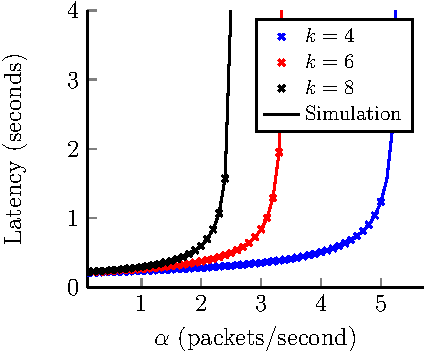
\includegraphics[width=\linewidth]{graphs/num_ports-crop}
	\caption{Latency predicted by the model and simulation for different numbers
of ports ($k$).} 
	\label{fig:num_ports}
\end{minipage}
\hfill
\begin{minipage}[b]{.49\textwidth}
	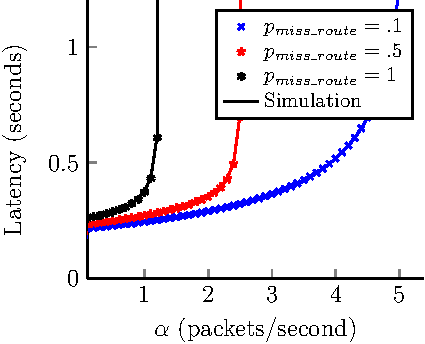
\includegraphics[width=\linewidth]{graphs/diff_sdn-crop}
	\caption{Latency predicted by the model and simulation with different
proportions of packets visiting the SDN controller ($p_{miss\_route}$).}
	\label{fig:sdn_perc}
\end{minipage}

\vspace{2mm}

\begin{minipage}[b]{.49\textwidth}
	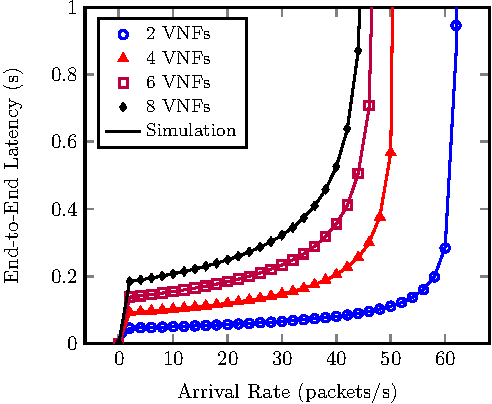
\includegraphics[width=\linewidth]{graphs/diff_lengths-crop}
	\caption{Latency predicted by the model and simulation for different length
service chains.}
	\label{fig:length_chain}
\end{minipage}
\hfill
\begin{minipage}[b]{.49\textwidth}
	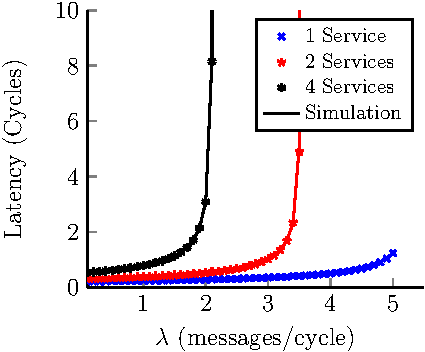
\includegraphics[width=\linewidth]{graphs/mult_services-crop}
	\caption{Latency predicted by the model and simulation for several services
with different length service chains.}
	\label{fig:mult_services}
\end{minipage}

\end{figure*}

To verify the accuracy of the analytical model, a discrete event simulator has been built using OMNeT++ \cite{VargaH08} to simulate a NFV and SDN enabled datacentre network. Each simulation experiment was run until the network reaches its steady state where further network cycles do not change the collected statistics appreciably.

Comprehensive simulation experiments were conducted to validate the performance of the proposed analytical model under different network configurations. However for the sake of specific illustration only a selection of tests are presented here and the results comparison between the analytical model and simulation experiments are presented in terms of the average end-to-end latency.

In practice a datacentre can contain on the order of tens of thousands of servers \cite{AWS16}, with each switch supporting 1 to 100Gbits/s traffic a second. Unfortunately it is computationally expensive to simulate a datacentre at this scale, especially for a large number of tests. Hence a scaled down version of a typical datacentre is modelled with the following parameters:

\begin{itemize}
\item $k = 4$, $k_{vsw} = 2$ and $p_{miss\_route} = 0$
\item The service rate of the switches and SDN controller are set to be 40 packets per second ($\mu_{sw} = 40$, $\mu_{sdn} = 40$)
\item The service rate of the VNFs is set to be 20 packets per second ($\mu_{vnf} = 20$)
\item Services are selected with equal probability
\item Case I: The network holds one service with two VNFs
\item Case II: The network holds multiple services and the number of VNFs in the $i$th service chain has a length of $i+1$
\end{itemize}

Figs \ref{fig:num_ports} to \ref{fig:mult_services} depict mean message latency predicted by the model plotted against those provided by simulation experiments for a range of parameter settings. For the model, results are only shown where the network is in a steady state, i.e. where the arrival rate is lower than or equal to the service rate for all queues. The figures demonstrate that the simulation results closely match those predicted by the model. The tractability and accuracy of the analytical model make it suitable for analysis of next generation NFV and SDN enabled Mobile Cloud computing datacentres.